% This is the Reed College LaTeX thesis template. Most of the work
% for the document class was done by Sam Noble (SN), as well as this
% template. Later comments etc. by Ben Salzberg (BTS). Additional
% restructuring and APA support by Jess Youngberg (JY).
% Your comments and suggestions are more than welcome; please email
% them to cus@reed.edu
%
% See http://web.reed.edu/cis/help/latex.html for help. There are a
% great bunch of help pages there, with notes on
% getting started, bibtex, etc. Go there and read it if you're not
% already familiar with LaTeX.
%
% Any line that starts with a percent symbol is a comment.
% They won't show up in the document, and are useful for notes
% to yourself and explaining commands.
% Commenting also removes a line from the document;
% very handy for troubleshooting problems. -BTS

% As far as I know, this follows the requirements laid out in
% the 2002-2003 Senior Handbook. Ask a librarian to check the
% document before binding. -SN

%%
%% Preamble
%%
% \documentclass{<something>} must begin each LaTeX document
\documentclass[12pt,twoside]{reedthesis}
% Packages are extensions to the basic LaTeX functions. Whatever you
% want to typeset, there is probably a package out there for it.
% Chemistry (chemtex), screenplays, you name it.
% Check out CTAN to see: http://www.ctan.org/
%%
\usepackage{graphicx,latexsym}
\usepackage{amsmath}
\usepackage{amssymb,amsthm}
\usepackage{longtable,booktabs,setspace}
\usepackage{chemarr} %% Useful for one reaction arrow, useless if you're not a chem major
\usepackage[hyphens]{url}
% Added by CII
\usepackage{hyperref}
\usepackage{lmodern}
\usepackage{float}
\floatplacement{figure}{H}
% End of CII addition
\usepackage{rotating}

% Next line commented out by CII
%%% \usepackage{natbib}
% Comment out the natbib line above and uncomment the following two lines to use the new
% biblatex-chicago style, for Chicago A. Also make some changes at the end where the
% bibliography is included.
%\usepackage{biblatex-chicago}
%\bibliography{thesis}


% Added by CII (Thanks, Hadley!)
% Use ref for internal links
\renewcommand{\hyperref}[2][???]{\autoref{#1}}
\def\chapterautorefname{Chapter}
\def\sectionautorefname{Section}
\def\subsectionautorefname{Subsection}
% End of CII addition

% Added by CII
\usepackage{caption}
\captionsetup{width=5in}
% End of CII addition

% \usepackage{times} % other fonts are available like times, bookman, charter, palatino

% Syntax highlighting #22

% To pass between YAML and LaTeX the dollar signs are added by CII
\title{A dissertation}
\author{Jessica L. Burnett}
% The month and year that you submit your FINAL draft TO THE LIBRARY (May or December)
\date{2019}
\division{}
\advisor{Craig R. Allen}
\institution{University of Nebraska-Lincoln}
\degree{Doctor of Philosophy}
%If you have two advisors for some reason, you can use the following
% Uncommented out by CII
\altadvisor{Dirac Twidwell}
% End of CII addition

%%% Remember to use the correct department!
\department{School of Natural Resources}
% if you're writing a thesis in an interdisciplinary major,
% uncomment the line below and change the text as appropriate.
% check the Senior Handbook if unsure.
%\thedivisionof{The Established Interdisciplinary Committee for}
% if you want the approval page to say "Approved for the Committee",
% uncomment the next line
%\approvedforthe{Committee}

% Added by CII
%%% Copied from knitr
%% maxwidth is the original width if it's less than linewidth
%% otherwise use linewidth (to make sure the graphics do not exceed the margin)
\makeatletter
\def\maxwidth{ %
  \ifdim\Gin@nat@width>\linewidth
    \linewidth
  \else
    \Gin@nat@width
  \fi
}
\makeatother

\renewcommand{\contentsname}{Table of Contents}
% End of CII addition

\setlength{\parskip}{0pt}

% Added by CII

\providecommand{\tightlist}{%
  \setlength{\itemsep}{0pt}\setlength{\parskip}{0pt}}

\Acknowledgements{
Graduate school itself isn't hard, but the journey is. I have a lot of people and institutions to thank for their emotional, intellectual, financial, and other professional support. I wish to first highlight how \textbf{great it was to be a graduate student at this university and in the School of Natural Resources}. I have received tremendous support at all levels of the university. Although I am not a fan of Nebraska's climate, I highly recommend this school to prospective students.
First, I thank my supervisors, Craig Allen and Dirac Twidwell, for providing me with this amazing opportunity and for supporting my growth as an independent researcher. I thank my committee members, Craig Allen, David Angeler, John De Long, Dirac Twidwell, and Drew Tyre for their support and advisement, but especially for their comprehensive examination--I found this process transformative. I especially thank Dirac for his comprehensive exam questions--I never knew how much theory I didn't know until I studied your list\ldots{}
\textbf{Financial support}. This research was funded by the U.S. Department of Defense's Strategic Environmental Research and Development Program (project ID: RC-2510). The University of Nebraska-Lincoln (UNL) has been highy supportive in my doctoral studies and reserach. I am grateful for the generous of donors to the University of Nebraska Foundation, which provided me with two prestigious supplemental fellowships: Fling and Othmer. I also thank the Nelson Family (Nelson Memorial Fellowship) and the Institute of Agriculture and Natural Resources, who funded large portions of my academic and research-related travel. I thank the School of Natural Resources for their financial support in my conference travel. The U.S. National Academy of Sciences generously funded part of my travel to the International Institute for Applied Systems Analysis (IIASA). This financial support provided me not only with invaluabe opportunities to attend and present at national and international conferences and workshops, conduct research abroad, and network--this funding alleviated some financial pressures associated with graduate school which allowed a more refined focus on my research. The opportunities and experiences provided to me by these funding sources were amazing, thank you all.
\textbf{Emotional support}. I am one of the many graduate students afflicted with mental health ``disorders'' which negatively impact my quality of life, at times. I am first grafteful to one friend who unknowingly destigmatized mental health, without which I may not have sought treatment and diagnosis--thank you, Hannah. Since my diagnoses, I have tried to encourage this destigmatization among graduate students in our department. I thank felow students and faculty who have also been outspoken regarding related issues (Jamilynn Polletto and Drew Tyre). Finally, I thank Terry Thomas for her patience, support, and knowledge as my general practitioner and mental health advocate.\\
I thank others for their various and probably unknowing contributions to my professional development: David Angeler, Christie Bahlai, Hannah Birge, Mary Bomberger Brown, John Carroll, Jenny Dauer, John DeLong, Tarsha Eason, Brian Fath, Ahjond Garmestani, Chris Lepczyk, Frank La Sorte, Chai Molina, Erica Stuber, Zac Warren, Lyndsie Wszola, Hao Ye, Peter Zebrowski.
I would like to especially thank some of the amazing and brilliant \textbf{female scientists} in my life for their encouragement: Jane Anderson, Hannah Birge, Mary Bomberger Brown, Tori Donovan, Brittany Dueker, Allie Schiltmeyer, Katie Sieving, Erica Stuber, and Lyndsie Wszola.
\begin{enumerate}
\def\labelenumi{\arabic{enumi}.}
\item
  \textbf{Federal employment}. One reason for coming to this program was specifically to study in a USGS Cooperative Research Unit, and to understand better life as a federal scientist. I thank Craig Allen and Kevin Pope for entertaining many hours of discussion (interrogation?) regarding federal employment.
\item
  \textbf{IIASA}. Studying at the International Institute for Applied Systems Analysis was an amazing opportunity. I thank Brian Fath and Elena Rovenskaya for their advisement, members of the Applied Systems Analysis research group for their feedback on my research, and to the postdocs and YSSPers.
\end{enumerate}
HEB, TD, CPR, DF, CRA, BF, ER, CAL, MPM, KES, FL, MBB,
\begin{enumerate}
\def\labelenumi{\arabic{enumi}.}
\tightlist
\item
  \textbf{Professional development}. AJT, KP, CRA, DT, MBB, JC,
\end{enumerate}
To my partner of eight years--Schultzie--thank you for everything. Just kidding, thank you, Nat Price.
}

\Dedication{
Something snarky to mike moulton -- maybe a limerick
}

\Preface{
Supplemental published materials include:
{[}1{]} DOD White paper on Fisher Information (include reference and post onto Zenodo, if not available via DOD webpage)
{[}2{]} Packages
{[}3{]} IIASA report
}

\Abstract{
THis is my amazing abstract.
}

% End of CII addition
%%
%% End Preamble
%%
%
\begin{document}

% Everything below added by CII
  \maketitle

\frontmatter % this stuff will be roman-numbered
\pagestyle{empty} % this removes page numbers from the frontmatter
  \begin{acknowledgements}
    Graduate school itself isn't hard, but the journey is. I have a lot of people and institutions to thank for their emotional, intellectual, financial, and other professional support. I wish to first highlight how \textbf{great it was to be a graduate student at this university and in the School of Natural Resources}. I have received tremendous support at all levels of the university. Although I am not a fan of Nebraska's climate, I highly recommend this school to prospective students.
    First, I thank my supervisors, Craig Allen and Dirac Twidwell, for providing me with this amazing opportunity and for supporting my growth as an independent researcher. I thank my committee members, Craig Allen, David Angeler, John De Long, Dirac Twidwell, and Drew Tyre for their support and advisement, but especially for their comprehensive examination--I found this process transformative. I especially thank Dirac for his comprehensive exam questions--I never knew how much theory I didn't know until I studied your list\ldots{}
    \textbf{Financial support}. This research was funded by the U.S. Department of Defense's Strategic Environmental Research and Development Program (project ID: RC-2510). The University of Nebraska-Lincoln (UNL) has been highy supportive in my doctoral studies and reserach. I am grateful for the generous of donors to the University of Nebraska Foundation, which provided me with two prestigious supplemental fellowships: Fling and Othmer. I also thank the Nelson Family (Nelson Memorial Fellowship) and the Institute of Agriculture and Natural Resources, who funded large portions of my academic and research-related travel. I thank the School of Natural Resources for their financial support in my conference travel. The U.S. National Academy of Sciences generously funded part of my travel to the International Institute for Applied Systems Analysis (IIASA). This financial support provided me not only with invaluabe opportunities to attend and present at national and international conferences and workshops, conduct research abroad, and network--this funding alleviated some financial pressures associated with graduate school which allowed a more refined focus on my research. The opportunities and experiences provided to me by these funding sources were amazing, thank you all.
    \textbf{Emotional support}. I am one of the many graduate students afflicted with mental health ``disorders'' which negatively impact my quality of life, at times. I am first grafteful to one friend who unknowingly destigmatized mental health, without which I may not have sought treatment and diagnosis--thank you, Hannah. Since my diagnoses, I have tried to encourage this destigmatization among graduate students in our department. I thank felow students and faculty who have also been outspoken regarding related issues (Jamilynn Polletto and Drew Tyre). Finally, I thank Terry Thomas for her patience, support, and knowledge as my general practitioner and mental health advocate.\\
    I thank others for their various and probably unknowing contributions to my professional development: David Angeler, Christie Bahlai, Hannah Birge, Mary Bomberger Brown, John Carroll, Jenny Dauer, John DeLong, Tarsha Eason, Brian Fath, Ahjond Garmestani, Chris Lepczyk, Frank La Sorte, Chai Molina, Erica Stuber, Zac Warren, Lyndsie Wszola, Hao Ye, Peter Zebrowski.
    I would like to especially thank some of the amazing and brilliant \textbf{female scientists} in my life for their encouragement: Jane Anderson, Hannah Birge, Mary Bomberger Brown, Tori Donovan, Brittany Dueker, Allie Schiltmeyer, Katie Sieving, Erica Stuber, and Lyndsie Wszola.
    \begin{enumerate}
    \def\labelenumi{\arabic{enumi}.}
    \item
      \textbf{Federal employment}. One reason for coming to this program was specifically to study in a USGS Cooperative Research Unit, and to understand better life as a federal scientist. I thank Craig Allen and Kevin Pope for entertaining many hours of discussion (interrogation?) regarding federal employment.
    \item
      \textbf{IIASA}. Studying at the International Institute for Applied Systems Analysis was an amazing opportunity. I thank Brian Fath and Elena Rovenskaya for their advisement, members of the Applied Systems Analysis research group for their feedback on my research, and to the postdocs and YSSPers.
    \end{enumerate}
    HEB, TD, CPR, DF, CRA, BF, ER, CAL, MPM, KES, FL, MBB,
    \begin{enumerate}
    \def\labelenumi{\arabic{enumi}.}
    \tightlist
    \item
      \textbf{Professional development}. AJT, KP, CRA, DT, MBB, JC,
    \end{enumerate}
    To my partner of eight years--Schultzie--thank you for everything. Just kidding, thank you, Nat Price.
  \end{acknowledgements}
  \begin{preface}
    Supplemental published materials include:
    {[}1{]} DOD White paper on Fisher Information (include reference and post onto Zenodo, if not available via DOD webpage)
    {[}2{]} Packages
    {[}3{]} IIASA report
  \end{preface}
  \hypersetup{linkcolor=black}
  \setcounter{tocdepth}{2}
  \tableofcontents

  \listoftables

  \listoffigures
  \begin{abstract}
    THis is my amazing abstract.
  \end{abstract}
  \begin{dedication}
    Something snarky to mike moulton -- maybe a limerick
  \end{dedication}
\mainmatter % here the regular arabic numbering starts
\pagestyle{fancyplain} % turns page numbering back on

\hypertarget{thesisdownthesis_word-default}{%
\chapter{thesisdown::thesis\_word: default}\label{thesisdownthesis_word-default}}

Placeholder

\hypertarget{preliminary-content}{%
\chapter*{Preliminary Content}\label{preliminary-content}}
\addcontentsline{toc}{chapter}{Preliminary Content}

Paste from index.rmd if knitting to git or html

\hypertarget{acknowledgements}{%
\section*{Acknowledgements}\label{acknowledgements}}
\addcontentsline{toc}{section}{Acknowledgements}

Paste from index.rmd if knitting to git or html

\hypertarget{preface}{%
\section*{Preface}\label{preface}}
\addcontentsline{toc}{section}{Preface}

Paste from index.rmd if knitting to git or html

\hypertarget{dedication}{%
\section*{Dedication}\label{dedication}}
\addcontentsline{toc}{section}{Dedication}

Paste from index.rmd if knitting to git or html

THis is my amazing abstract.

\hypertarget{intro-chapter}{%
\chapter{Introduction}\label{intro-chapter}}

Anthropogenic activity in the last few decades has drastically influenced the interations within and among Earth systems worldwide. The complexity of and drivers of changes in coupled human-natural systems is consequently altered, further limiting our ability to detect and predict change and impacts of change (Liu et al., 2007; Scheffer, 2009).

Early warning systems are developed to detect and predict abrupt changes in disparate systems, e.g.~cyber security {[}@{]}, infrastructure {[}@{]}, banking crises (Davis \& Karim, 2008), and agricultural systems {[}@{]}. The need to develop and improve early warning systems for natural and coupled human-natural systems is exacerbated by the consequences of climate change and globalization, especially when the human-related stakes are high.

\hypertarget{practicality-of-early-warning-systems}{%
\subsection{Practicality of early warning systems}\label{practicality-of-early-warning-systems}}

Forecasting change is arguably the holy grail of ecology. The ability to forecast change, paired with an understanding of system interactions, provides opportunity to prevent or mitigate systemic change. Despite the plethora of regime shift theory and proposed early warning systems in the ecological literatures, early warning systems are currently of limited practical utility. I explain this paradox as a function of early warning systems having the following qualit(ies):
1. system or context specific; not generalizable\\
1. require a large number of observations\\
1. difficult implementation\\
1. difficult interpretation\\
1. require an understanding of the drivers of change\\
1. perform poorly under uncertainty\\
1. give no uncertaintiy around estimates\\
1. ignore observation error\\
Research in these areas will improve existing and inform future early warning systems, such that they are useful to practitioners and other end-users. In this dissertation I tackle \textbf{THE ABOCE NUMBERS LIST HERE}.

\hypertarget{dissertation-aims}{%
\subsection{Dissertation aims}\label{dissertation-aims}}

The overarching aim of this work is to advance our understanding of the utility and limitation of using early warning systems (or regime detection metrics). Specifically, I examine those systems/models designed to detect abrupt change in ecological communities. This work is of value to both practitioners and theoreticians:
- Chapters are written as separate, publishable manuscripts (\emph{sans} literature cited) geared towards the theoretical and applied ecologist\\
- Case studies, statistical software, and data are provided as reproducible examples of select methodologies.

\hypertarget{chapter-rdmMethodsReview}{%
\chapter{A review of quantitative methods for identifying ecological regime shifts in ecological communities}\label{chapter-rdmMethodsReview}}

Placeholder

\hypertarget{introduction}{%
\section{Introduction}\label{introduction}}

\hypertarget{existing-rdms-in-ecological-literature}{%
\section{Existing RDMs in ecological literature}\label{existing-rdms-in-ecological-literature}}

\hypertarget{methods}{%
\subsection{Methods}\label{methods}}

\hypertarget{boolean-search}{%
\subsubsection{Boolean search}\label{boolean-search}}

\hypertarget{notes-on-the-boolean-search-in-wos}{%
\paragraph{Notes on the boolean search in WOS}\label{notes-on-the-boolean-search-in-wos}}

\hypertarget{removingretaining-papers-from-search}{%
\subsubsection{Removing/retaining papers from search}\label{removingretaining-papers-from-search}}

\hypertarget{wos-search-results}{%
\subsection{WOS Search results}\label{wos-search-results}}

\hypertarget{existing-rdm-and-related-review-articles}{%
\section{Existing RDM and related review articles}\label{existing-rdm-and-related-review-articles}}

\hypertarget{rdms-not-yet-explored-for-ecological-data}{%
\section{RDMs not yet explored for ecological data}\label{rdms-not-yet-explored-for-ecological-data}}

\hypertarget{methods-1}{%
\section{Methods}\label{methods-1}}

\hypertarget{identifying-papersrsdms-in-the-literature}{%
\subsection{Identifying papers/RSDMs in the literature}\label{identifying-papersrsdms-in-the-literature}}

\hypertarget{results}{%
\section{Results}\label{results}}

\hypertarget{potential-figures}{%
\subsection{Potential figures}\label{potential-figures}}

\hypertarget{potential-tables}{%
\subsection{Potential tables}\label{potential-tables}}

\hypertarget{discussion}{%
\section{Discussion}\label{discussion}}

\hypertarget{fiGuide}{%
\chapter{A guide to Fisher Information for Ecologists}\label{fiGuide}}

\hypertarget{abstract}{%
\section{Abstract}\label{abstract}}

Ecological regime shifts are increasingly prevalent in the Anthropocene. The number of methods proposed to detect these shifts are on the rise yet few are capable detecting regime shifts without a priori knowledge of the shift or are capable of handling high-dimensional and noisy data. A variation of Fisher Information (FI) in a dataset was proposed as a method for detecting changes in the orderliness of ecological systems. Although FI has been described in multiple research articles, previous presentations do not highlight a key component of FI that may make the metric easier to understand by practitioners. We use a two-species predator prey model to describe the concepts required to calculate FI. We hope this work will serve as a useful explanation of the FI metric for those seeking to understand it in the ecological systems and regime shifts.

\hypertarget{introduction-1}{%
\section{Introduction}\label{introduction-1}}

Changes in the feedback(s) governing ecosystem processes can trigger unexpected and sometimes undesirable responses in environmental conditions (Scheffer, Carpenter, Foley, Folke, \& Walker, 2001; Walther et al., 2002). Ecologists often refer to such changes as regime shifts---but this term is used interchangeably in the literature with state change, state transition, or alternative state (Andersen, Carstensen, Hernández-García, \& Duarte, 2009). Climate change and globalization are triggering novel and unexpected changes in ecosystems, and the rapidity with which these changes occur make predictive modeling difficult. Although detecting regime shifts becomes more difficult as we increase the extent and complexity of the system in question , advances in the collection and analysis of ecological data may improve our ability to detect impending regime shifts in time for intervention (Jorgensen \& Svirezhev, 2004).

Although multiple quantitative approaches are proposed as regime shift detection methods ,few are consistently applied to terrestrial ecological data. We classify a regime shift detection methods (DMs) broadly as either model-based or model-free (Boettiger \& Hastings, 2012; Dakos et al., 2012; Hastings \& Wysham, 2010). Model-based methods incorporate mathematical (mechanistic) representations of the system (Hefley, Tyre, \& Blankenship, 2013) and carry strict assumptions, which are often violated by real systems (Abadi, Gimenez, Arlettaz, \& Schaub, 2010). In addition to assumption violations nullifying parts of the model, model misspecification may yield spurious results {[}Perretti, Munch, \& Sugihara (2013).

Model-free (or metric-based detectin ethods (e.g., descriptive statistics, cross-correlation mapping) require fewer assumptions to implement than do model-based DMs (Dakos et al., 2012). The most widely used model-free methods for detecting ecological regime shifts include descriptive statistics of one or a few components of a system, such as variance, skewness, and mean value (Andersen et al., 2009; Mantua, 2004; Rodionov \& Overland, 2005) and composite measures which handle multivariable data, including principal components analysis (Petersen et al., 2008), clustering algorithms (Beaugrand, 2004), exergy (Fath \& Cabezas, 2004), and Fisher Information (Cabezas \& Fath, 2002; Karunanithi, Cabezas, Frieden, \& Pawlowski, 2008).

Fisher Information, hereafter FI is a model-free composite measure of any number of variables (Fisher, 1922), and is proposed as an early warning signal for ecological regime shift detection system sustainability (Mayer, Pawlowski, Fath, \& Cabezas, 2007, p. @karunanithi\_detection\_2008, Eason and Cabezas 2012, Eason et al.~2014a). Three definitions of FI exist:
I. A measure of the ability of the data to estimate a parameter.\\
II. The amount of information extracted from a set of measurements {[}Roy Frieden (1998); frieden\_fisher\_1990{[}{]}.\\
III. A measure representing the dynamic order/organization of a system (Cabezas \& Fath, 2002).

The application of FI to complex ecological systems was posed as part of the `Sustainable Regimes Hypothesis,' stating a system is sustainable, or is in a stable dynamic state, if over some period of time the average value of FI does not drastically change (Cabezas \& Fath, 2002). This concept can be described using an ecological example. Consider the simple diffusion of a population released from a point source at \(t = 0\). This process can be described by a bivariate normal distribution, \(p(x,y\vert t)\). As the time since release (as \(t\) increases) increases the spread of the distribution, \(p(x,y\vert t)\), becomes larger (less concentrated about the mean) because the animals have moved further from the release location. FI will decrease in value as t increases, because \(p(x,y\vert t)\) contains less information (higher uncertainty) about where the animals will be located. As \(t→\infty\), the animals will be relatively uniformly distributed across the environment and \(p(x,y\vert t)\) will carry no information about the location of the animals. Consequently, as \(t→\infty\), FI will approach zero. This system is not in a stable dynamic state because FI is decreasing with time.

In contrast, imagine a population varying around a carrying capacity following a simple logistic growth model. As long as the average system parameters (r and K and their variances) are stationary (not changing with time), then the logarithm of population size will have a normal distribution (check this -- might need some different model). The FI measured over any selected window of time will be constant, indicating that the system is in a stable dynamic state. A perturbation to the population size due to disturbance will also not affect FI, as long as the disturbance does not change the distributions of r and K, and the perturbations themselves occur with some stationary probability distribution.

Although the concept of FI is firmly grounded in physics (Frieden, 1998), the concepts behind its application to ecological systems remain elusive to the average ecologist. We aim to elucidate the statistical concept of FI and the steps required to calculate it as a measure of `ecosystem order' and as a regime shift detection method (Cabezas \& Fath, 2002; Fath, Cabezas, \& Pawlowski, 2003). We believe a concise and accessible synthesis of the topic, along with reproducible code, will aid the ecologists' understanding of this metric and will advance our understanding of its usefulness as an indicator of ecological regime shifts. We reproduce the analyses presented in (Fath et al., 2003) and Mayer et al. (2007) to fully explain these concept of and steps for calculating this form of Fisher Information. We hope this work will serve as a useful explanation of the FI metric for those seeking to understand it in the ecological regime shift context and will stimulate research using this and other multivariate, model-free, and composite measures to understand ecological regime shifts.

\#\#\#On Fisher Information
Two methods exist for calculating Fisher Information (FI) as applied to ecological systems data, which we refer to as the `derivatives-based' method, first appearing in Cabezas \& Fath (2002), and the `binning' method, first appearing in Karunanithi et al. (2008). The binning method was proposed as an alternative to the derivatives-based method for handling noisy and sparse data, and requires additional calculations and system-specific decisions, and for these reasons we focus solely on the derivatives-based method. The general form of FI can be found in (Fath et al., 2003) and (Mayer et al., 2007), and although others can be found, we refer the reader to Cabezas \& Fath (2002) for a complete derivation of FI, and to @ref(\#fiBiblio) for applications of Fisher Information in other fields.

\#\#\#Notation\\
A capital letter (e.g., \(A\)) denotes a random variable; an asterisk superscript (\(^*\)) indicate a particular realization; \emph{bold notation} indicates that the state of the system is defined in more than one dimension.

\#\#\#Steps for calculating Fisher Information (FI)
To calculate FI for a system with more than one state variable, we first estimate the probability of observing the system \(p(x)\) in a given state, \(x\), over time period \(T\). The probability density function, \(p(x)\), is then directly used to calculate the derivatives-based FI. We use bold notation to indicate that the state of the system is defined in more than one dimension (e.g., the state of a predator prey system is defined in two dimensions by the number of predators and number of prey). Here, we describe these steps and present the numerical calculation of FI using a two-species predator-prey model {[}Fath et al. (2003); mayer\_applications\_2007{]}, hereafter referred to as the `model system':
\begin{equation} 
  dx_1 = g_{1}x_{1}(1-\frac{x_1}{k})- \frac{l_{12} x_{1} x_{2}}{1+\beta x_{1}} \\
  dx_2 = \frac{g_{21}x_1 x_2}{1+\beta x_1} - m_2 x_2) \\
  \label{eq:predprey}
\end{equation}
The specified parameters for the model system are \(g_1=m_2=1\), \(l_12=g_12 = 0.01\) , \(k=625\) ,and \(\beta=0.005\) (see Fath et al., 2003; Frieden \& Gatenby, 2007; Mayer et al., 2007). The initial conditions (predator and prey abundances) for the model system were not provided in the original references. Using package \emph{deSolve} in Program R (v 3.3.2) to solve the model system \eqref{eq:predprey} we found \(x_1 = 277.7815\) and \(x_1= 174.551\) provided reasonable results. We found that a complete cycle of the system corresponds to approximately 11.145 time units.
\begin{figure}
\centering
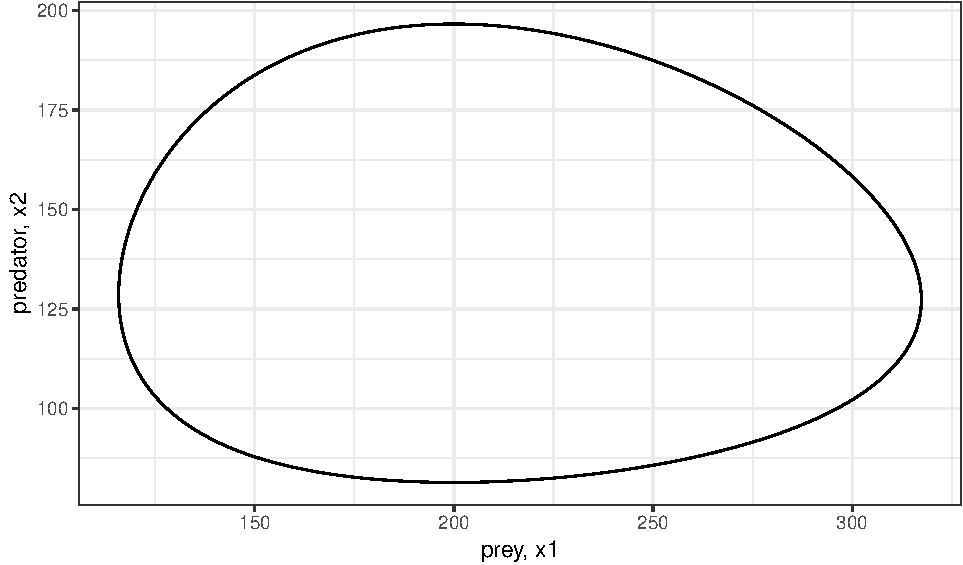
\includegraphics{myDissertation_files/figure-latex/pp1Period-1.pdf}
\caption{\label{fig:pp1Period}Phase space plot of two-species Lotka-Volterra predator-prey system over a single period (\textasciitilde{}11.145 time units.}
\end{figure}
\#\#\#Concepts behind the calculations\\
Although the numerical steps for calculating the derivatives-based FI are relatively straightforward, the concepts required to interpret the measure in the context of multiple variables is more complex. Here, we thoroughly discuss the concepts and assumptions behind FI calculation. Below, steps do not represent steps within the calculation, they represent the major concepts required

\#\#\#\#\textbf{Step 1. Probability of observing the system in a particular state, \(p(x)\)}\\
Fisher Information (FI) is defined with respect to a probability distribution. In the derivatives-based method, FI is calculated for a probability of observing a system (as defined by one or more state variables) in a particular state, \(p(x)\), over some period of time, (\(0 to t_{end}\)). In other words \(p(x)\) is the probability that, at a specific point in time (\(t_{obs}^*\)) we will observe the system in a particular state, \(x^*\). The time at which we observe the system is a random variable, \(t_{obs} ~ Uniform(0,t_{end})\). To be clear, the study system is assumed to be deterministic and we assume no observation error, however, the observed state of the system, \(x(T_{obs})\), is a random variable because it is a function of the random observation time, \(x^*= x(t_{obs}^*)\). The state of the model system, x, is defined in two dimensions by the number of predators and the number of prey \eqref{eq:predprey} and is easily visualized \ref{fig:pp1Period}.Therefore, the probability of observing a particular state is a two-dimensional joint distribution \ref{fig:2d-hist}.
\begin{figure}
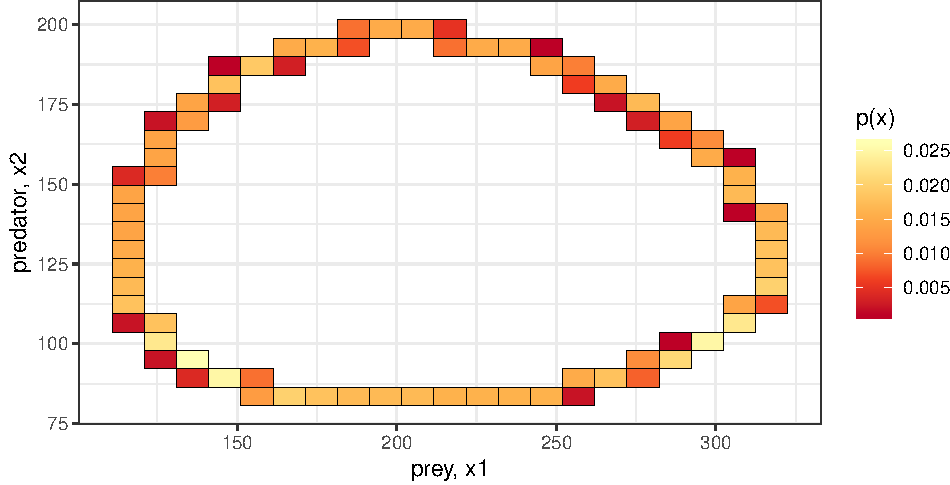
\includegraphics[width=0.85\linewidth]{myDissertation_files/figure-latex/2D-hist-1} \caption{A 2-dimensional histogram of the probability of observing a system in a particular state, $p(x)$, of the 2-species Lotka-Volterra predator prey system over a single period (~11.145 time units).}\label{fig:2D-hist}
\end{figure}
A single state of the model system is defined by the number of predators and prey at a given point in time such that for any given point in time \(x(t)=[x_1 (t),x_2 (t)]\). At some random time between 0 and \(t_{end}\) {[}\(T_{obs} ~ Uniform(0,t_{end})\){]} we can count the number of predators and the number of prey to determine the state of the model system. We must assume the system is deterministic and there is no observation error. We can then calculate the probability of observing a particular predator and prey abundance combination, \(p(x)\). Under these assumptions, the only possible states of the system are defined by the system's observed trajectory, the model parameters, and the initial conditions. Therefore, the support of the probability distribution \ref{fig:2D-hist} is the trajectory of the system.
\begin{figure}
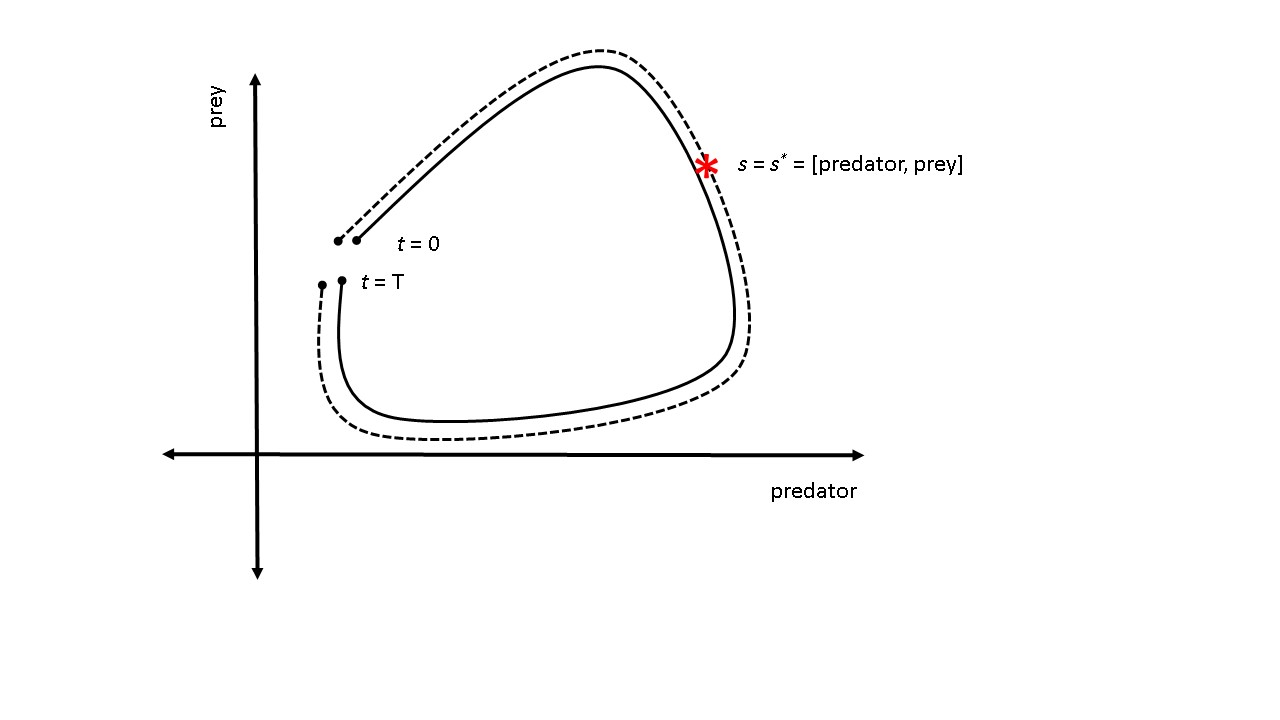
\includegraphics[width=1\linewidth]{./chapterFiles/fiGuide/figures/stringFig} \caption{A single cycle of a hypothetical two-species system over time period $t = 0$ to $t = T$. $s^*$ is the state of the system at some point in time. The dotted line represents the distance travelled by the system in phase space over its trajectory during time $(0, T)$.}\label{fig:stringFig}
\end{figure}
\#\#\#\#\textbf{Step 2.} Distance traveled by the system, \(s\)
Distance traveled by the system, s. We can now move from an n-dimensional representation of the probability distribution to a one-dimensional representation. To better understand this, imagine placing a string over the path of the entire trajectory from \(0 to t_{end}\) \ref{fig:stringFig}. If we know the number of predators and prey at a particular point in time \((t_{obs}^*)\) then we can mark that location on the string (see asterisk in \ref{fig:stringFig}. Next, imagine picking up the string and laying the string flat along a ruler. The length, s, of the entire string measures the total distance traveled by the system in phase space. The mark we made on the string (denoted \(*\)) lies at a distance \(s^*\) between 0 and \(s\). We call this length the distance traveled by the system, \(s^*\). In this context, \(s^*\) in phase space represents a measure of cumulative change in state. We note that the distance traveled in phase space increases monotonically with time. If the system never revisits the same state (i.e., the trajectory never overlaps or intersects itself), then every unique system state (i.e., point on the trajectory) is mapped to a unique value of distance traveled. Therefore, \(p(x)\) (n-dimensional) is equivalent to the probability that the system is at distance s, i.e., \(p(x)=p(s)\), (where \(p(s)\) is one dimensional; Cabezas, Pawlowski, Mayer, \& Hoagland (2005)). However, if the system revisits previous states, then a unique system state may be mapped to different values of distance traveled and the relationship between \(p(x)\) and \(p(s)\) is not one-to-one. We calculated the distance traveled s of the model system over a single cycle (11.145 time units; \ref{fig:distSpeedAccel}.
\begin{figure}
\centering
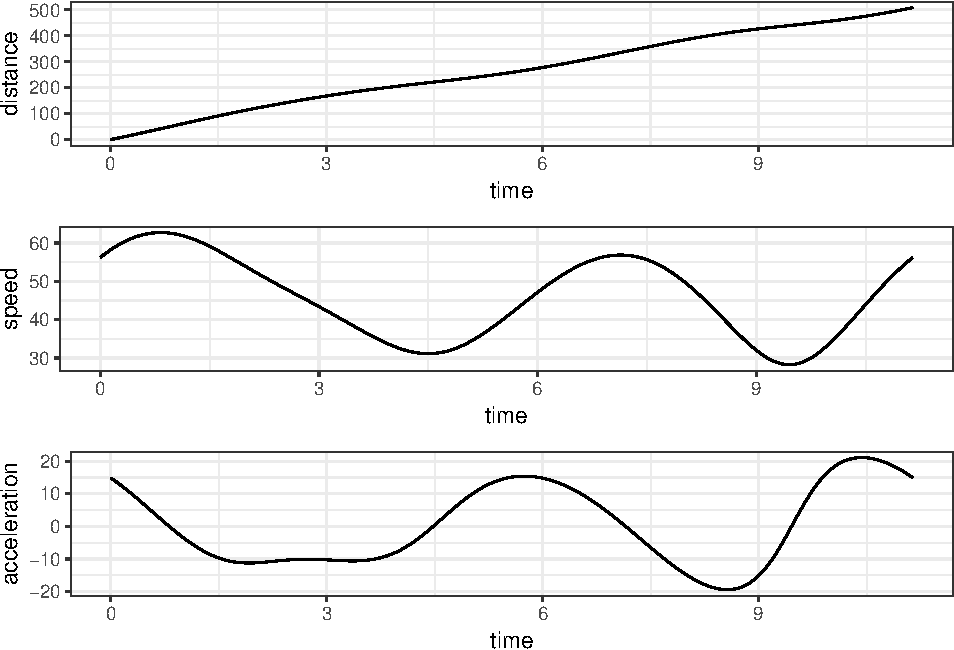
\includegraphics{myDissertation_files/figure-latex/distSpeedAccel-1.pdf}
\caption{\label{fig:distSpeedAccel}From top to bottom, distance traveled in phase space, speed tangential to system trajectory, acceleration tangential to system trajectory.}
\end{figure}
\hypertarget{step-3.-ps-as-a-function-of-the-rate-of-change-of-s}{%
\subsubsection{\texorpdfstring{\textbf{Step 3.} \(p(s)\) as a function of the rate of change of \(s\)}{Step 3. p(s) as a function of the rate of change of s}}\label{step-3.-ps-as-a-function-of-the-rate-of-change-of-s}}

In previous presentations of FI, the relationship between the state of the system (n-dimensional) and the distance traveled (1-dimensional) was not always emphasized (Cabezas \& Fath, 2002). Here we use x to denote the state of the system and s to denote the distance traveled to emphasize this distinction. If a system travels at a constant speed over the entire time period, then the system is equally likely to be in any state along the trajectory (\(s\) is linear and \(p(s)\) is uniform). Referring to our model system, if the number of predators and prey are linearly related, then the speed of the system is constant. For non-linear systems, the distribution above the string will not be uniform \ref{fig:stringFig}. Rather, it will change depending on the amount of time the system spends in each state. It follows that \(p(s)\) is proportional to the inverse of the rate of change of distance traveled (i.e., the speed along the path in phase space).

We will now demonstrate this using our model system as an example. Suppose the abundances of the predator and their prey in our model system predictably operate at carrying capacity. Over a relatively short period of time the prey abundance quickly declines after a severe weather event (a pulse disturbance; (Bender et al.~1984), but quickly recovers. Intuitively, the absolute rate of change at time points near the disturbance will be larger than during time periods long before or long after the disturbance. It is therefore more likely that the system will be (observed) in a state where prey and predators are operating approximately at carrying capacity than in a state with relatively low prey abundance. Mathematically, the time, \(t*\), at which we calculate the abundances of prey and predators is a uniform random variable, and the distance traveled by the system, \(s^*\), is a function of time, is differentiable, and monotonically increases. Therefore, the probability density function of the distance traveled \(p(s)=\frac{1}{T}\frac{1}{s'}\), where \(s'= \frac{ds}{dt}\) is the speed of the system (the speed tangential to the trajectory; the first derivative of the distance traveled; instantaneous rate of change of \(s\)). We calculated the speed (the first derivative; \ref{fig:distSpeedAccel} and acceleration (the second derivative; \ref{fig:distSpeedAccel} of the distance traveled s by the model system over a single cycle using function ode in package deSolve (Soetaert et al.~2010) in Program R (R Core Team 2016).

\hypertarget{step-4.-calculate-the-derivatives-based-fisher-information}{%
\subsubsection{\texorpdfstring{\textbf{Step 4.} Calculate the derivatives-based Fisher Information}{Step 4. Calculate the derivatives-based Fisher Information}}\label{step-4.-calculate-the-derivatives-based-fisher-information}}

Now that we understand how to calculate both the distance traveled, \(s\), and its probability density, \(p(s)\), calculating the derivatives-based FI is straightforward and computationally inexpensive \eqref{eq:fiDerivs}. There are several comparable equations for calculating the shift-invariant FI, and some may offer numerical advantages over others. Equation \eqref{eq:fiAdapted} is the general form and Equation \eqref{eq:fi73c} is the amplitude form for FI (in Mayer et al. (2007), respectively). Although these formulations are equivalent, \eqref{eq:fi73c} is most readily calculated when the differential equations for the system are known, obviating any advantage of a model-free metric.
\begin{equation}   
    I = \frac{1}{T} \int_0^T dt\left[\frac{s''^2}{s'^4}\right]^2 \\  
  \label{eq:fiDerivs}  
\end{equation}
\begin{equation} 
    I = \int \frac{ds}{p(s)}\left[\frac{dp(s)}{ds}\right]^2  \\
    \label{eq:fiAdapted}
\end{equation}
\begin{equation} 
    I = 4 \int ds\left[\frac{dq(s)}{ds}\right]^2 \\
\label{eq:fi73c}
\end{equation}
This article is interested in the Fisher Information calculated for a distribution of distance traveled, \(s\), by the entire system. We calculated the Fisher Information value using Equation \eqref{eq:fiDerivs} over a single period of the model system (\ref{predprey}). We calculated Fisher Information to be \(5.3\) x \(10^{-5}\) which is consistent with the results of Mayer et al.~(2007).

\#\#Case Study\\
Mayer et al.~(2007) calculated FI for a predator-prey system for several discrete values of carrying capacity of prey. The results of this study showed that FI was different for systems with different carrying capacities. However, this study did not address the central question of how FI changes during a regime shift. As an extension of the original study, we simulate a regime shift by modeling a situation where carrying capacity is abruptly decreased. To simulate an abrupt change in carrying capacity, we assume carrying capacity is described by Eq. 6 where \(k1\) is the initial carrying capacity, \(k2\) is the final carrying capacity, \(t*\) is the time of the regime shift, and alpha is a parameter that controls how quickly the regime shift occurs. The hyperbolic tangent function simulates a smooth, continuous change in carrying capacity while still allowing for the change to occur suddenly. To incorporate the change in carrying capacity into the system differential equations we define the rate of change of carrying capacity as given by \eqref{eq:mayerCase}.\\
\begin{equation}  
  k(t) = k_1  - 0.5(k_1-k_2)(\tanh(\alpha (t-t^*))+1)     \\
  k'(t) = 0.5\alpha (k_1-k_2)(\tanh(\alpha(t-t^*))^2 +1)      \\ 
\label{eq:mayerCase}
\end{equation}
\begin{verbatim}
[1] 5.370485e-05
\end{verbatim}
\begin{verbatim}
[1] 5.371751e-05
\end{verbatim}
\begin{verbatim}
[1] 5.326461e-05
\end{verbatim}
\begin{figure}
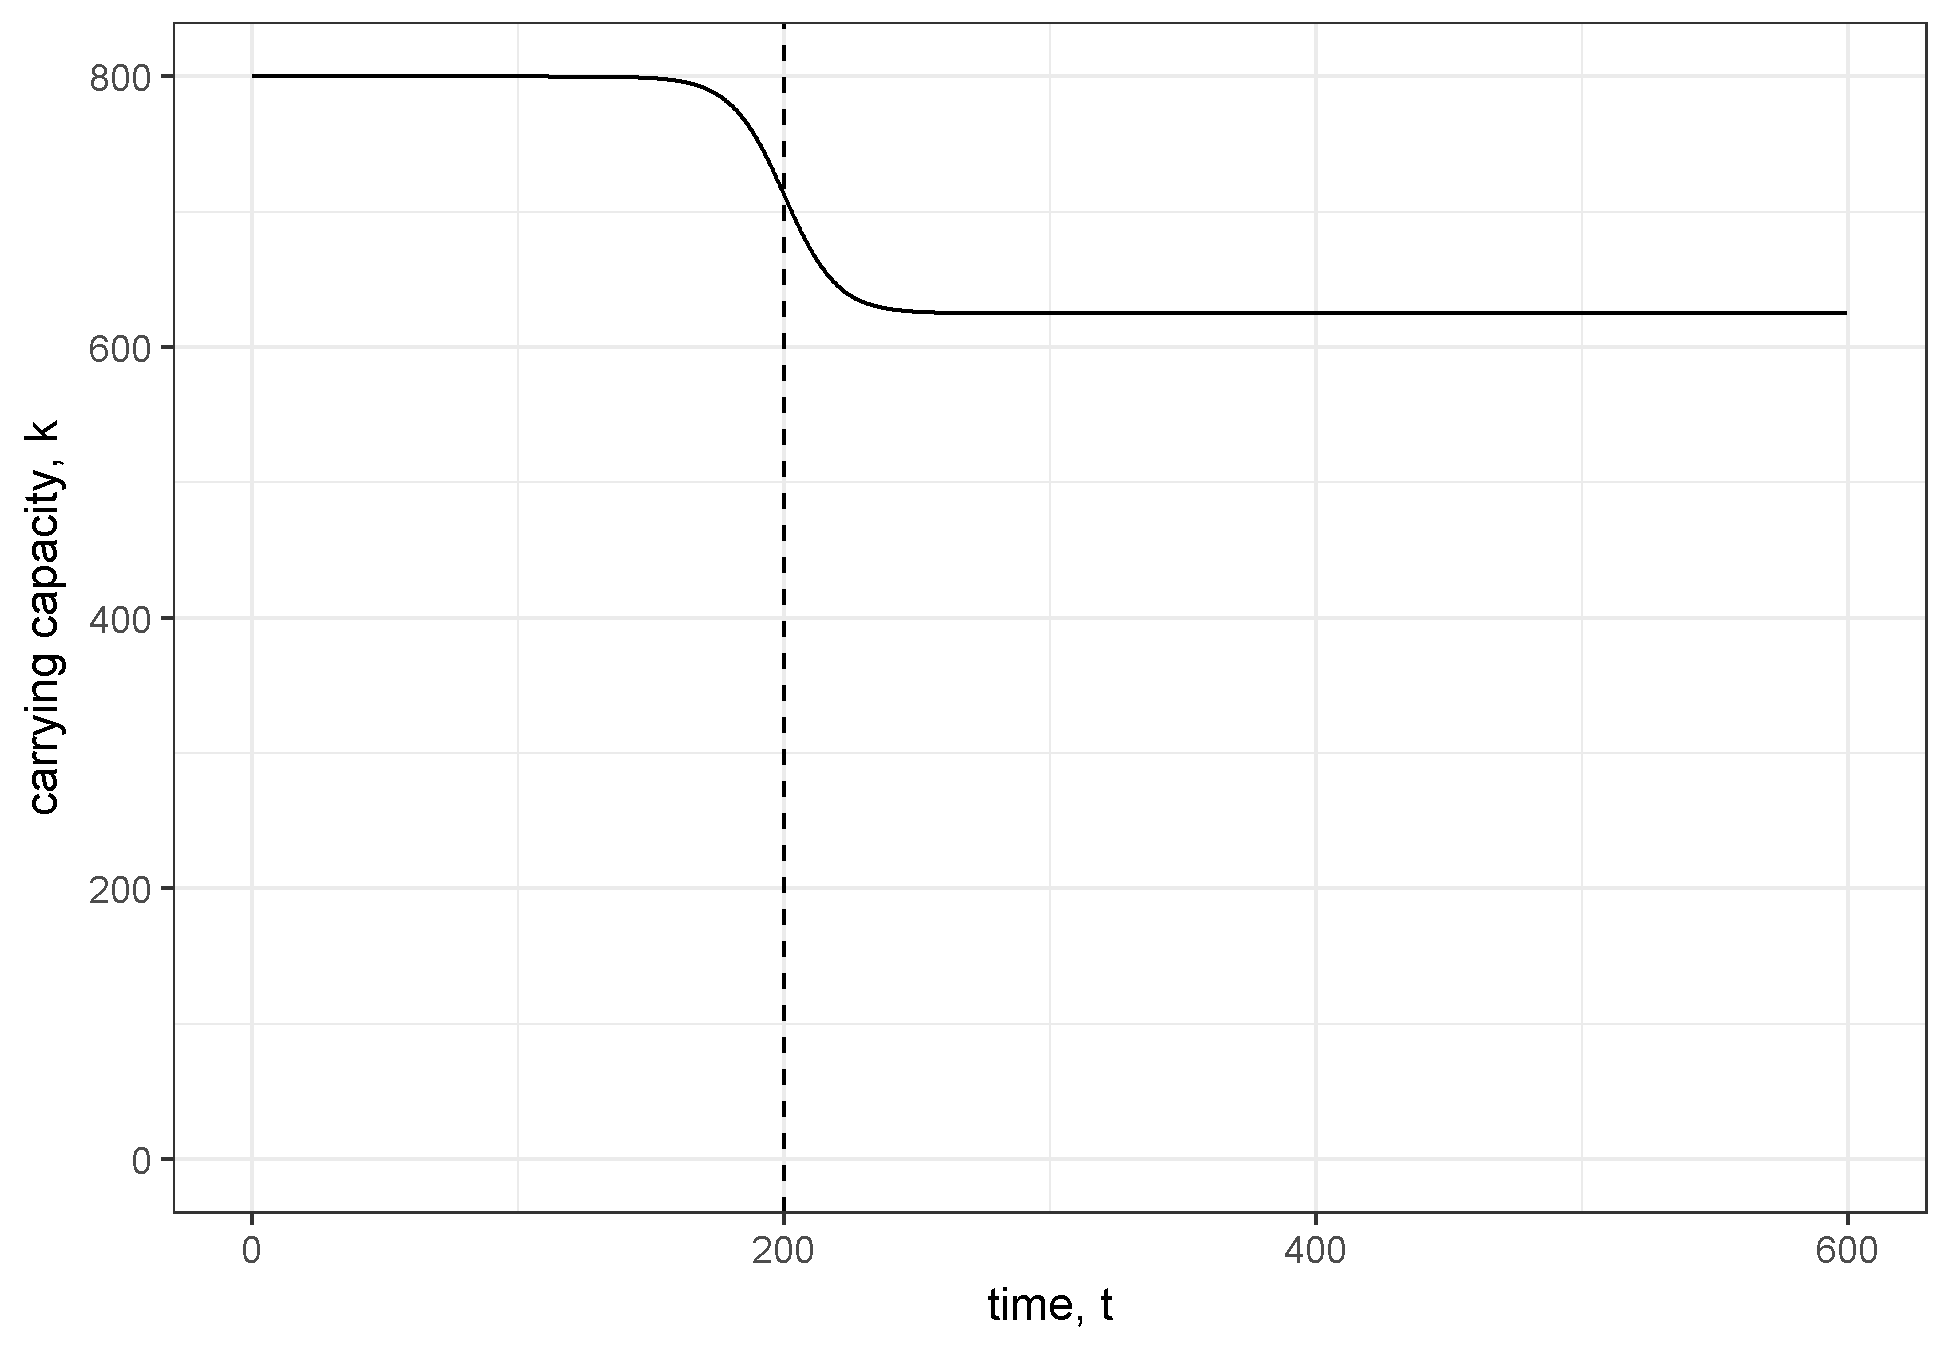
\includegraphics[width=1\linewidth]{./chapterFiles/fiGuide/figures/kByTime} \caption{Carrying capacity over time with a regime shift occuring around time 200.}\label{fig:kByTime}
\end{figure}
\begin{figure}
\centering
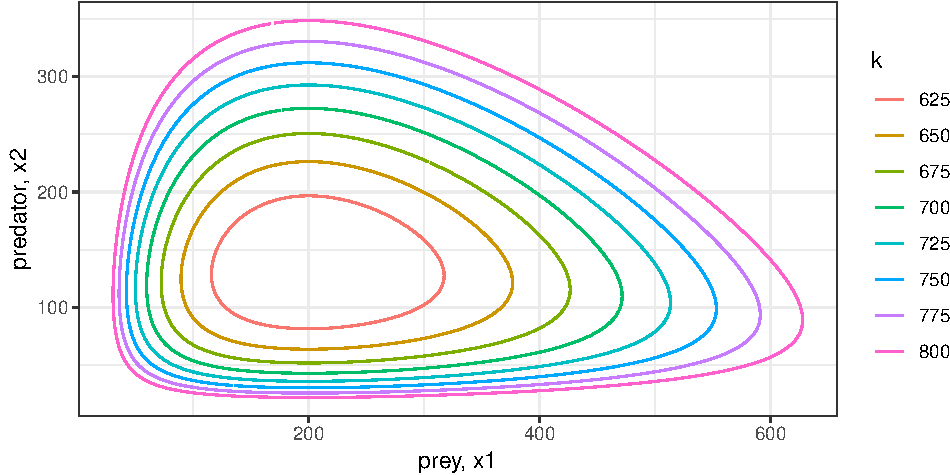
\includegraphics{myDissertation_files/figure-latex/kTrajectories-1.pdf}
\caption{\label{fig:kTrajectories}Phase space plot of system trajectories for different values of k}
\end{figure}
We assumed an initial carrying capacity of 800 and a final carrying capacity of 625 which corresponds to the range of carrying capacities explored by Mayer et al.~(2007). We simulated a time series of 600 time units with a regime change after 200 time units. We used an alpha value of 0.05. The time series for carrying capacity is shown in \ref{fig:kByTime} and the system trajectory in phase space is shown in \ref{fig:kTrajectories}. The distance travelled in phase space (i.e., cumulative change in state) is shown in \ref{fig:distOverTime} and the speed of the system (i.e., rate of change) is shown in \ref{fig:dsdtOverTime}.
\begin{figure}
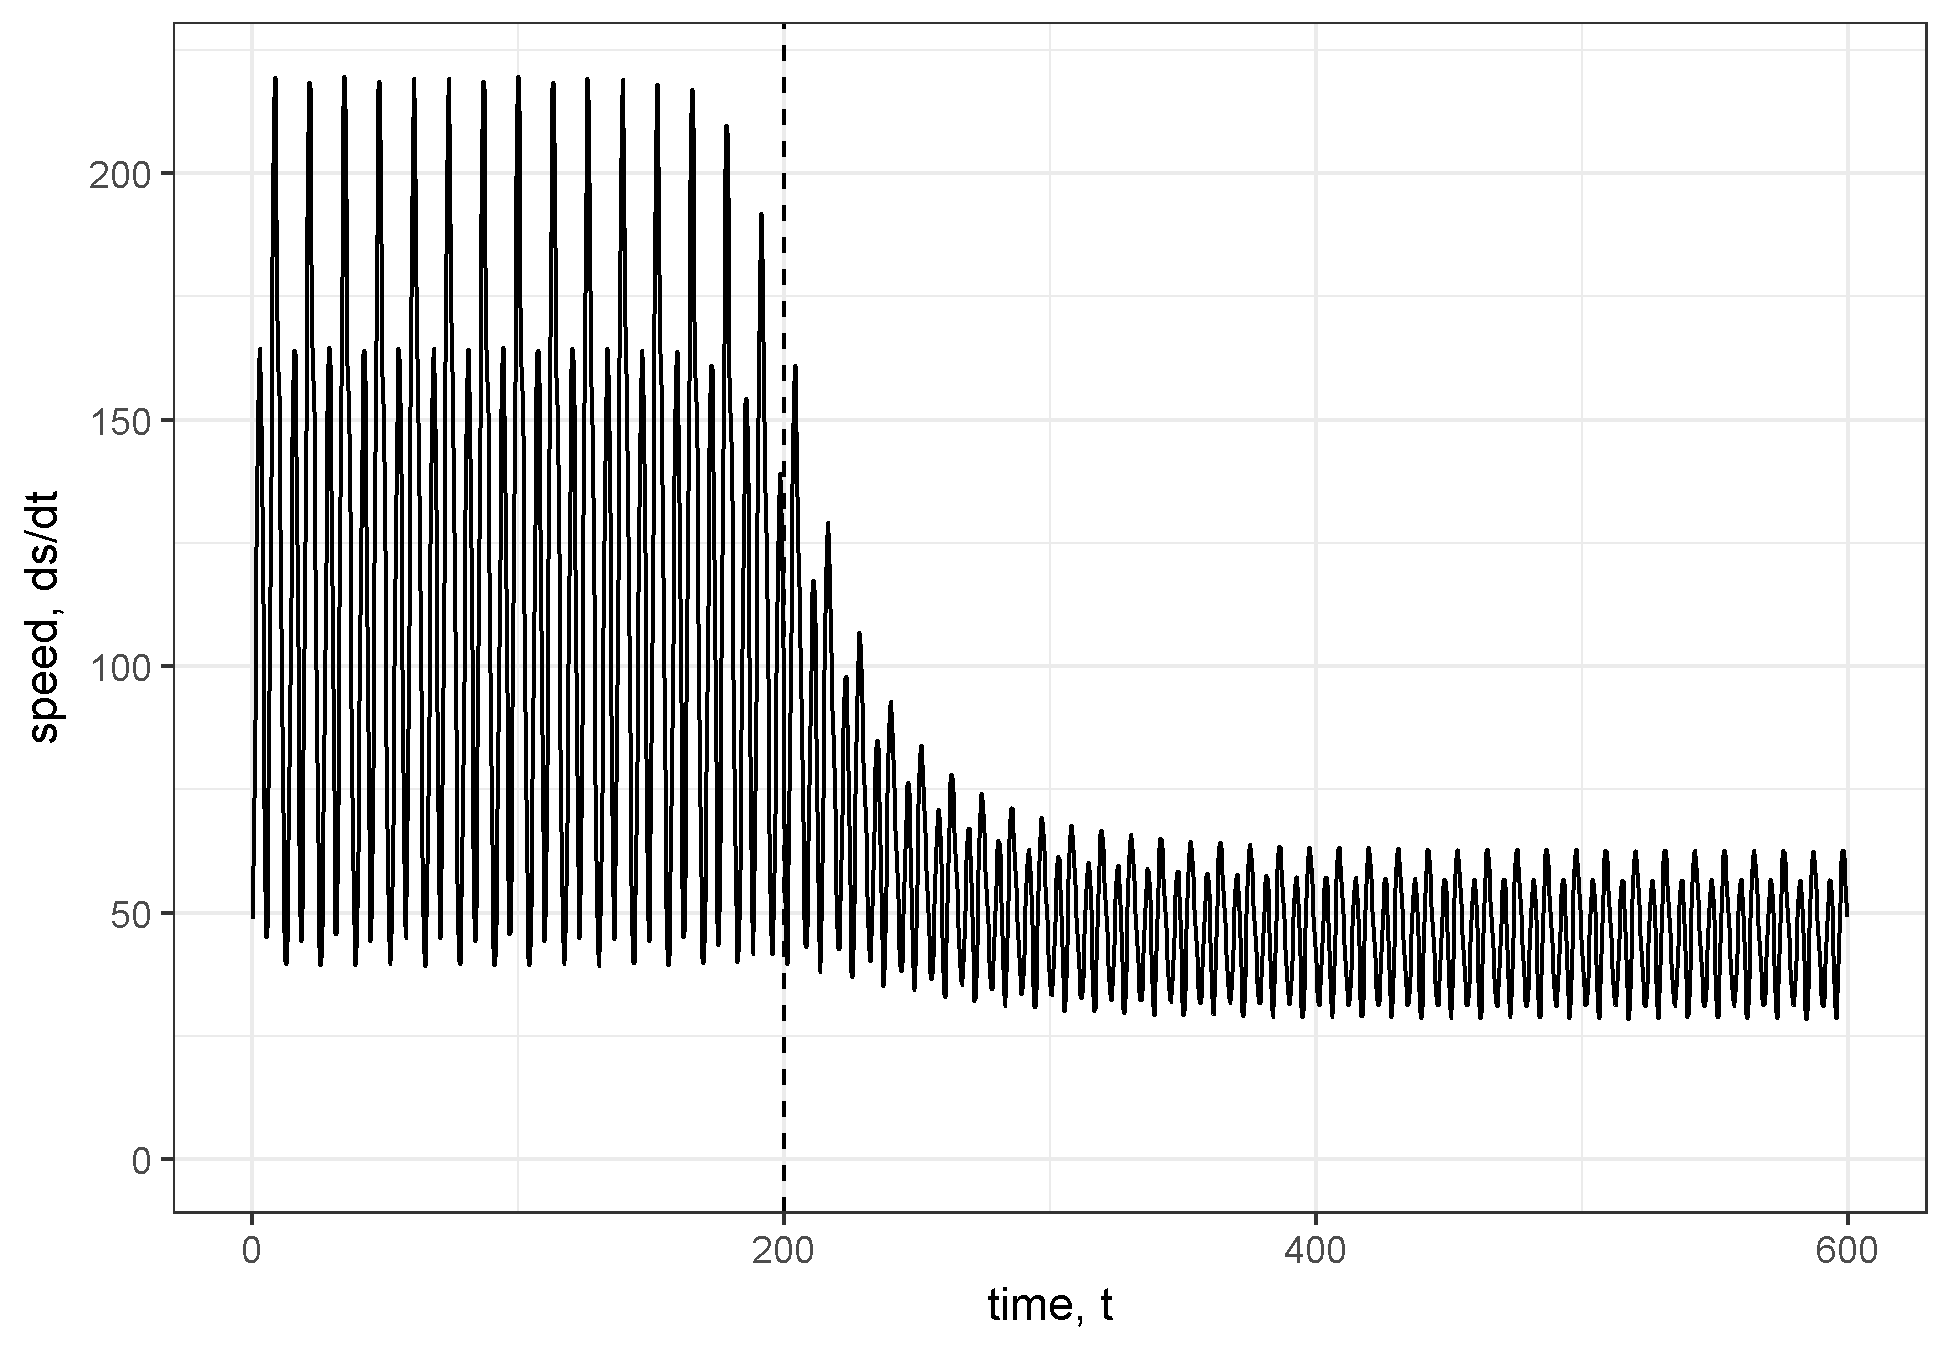
\includegraphics[width=0.85\linewidth]{./chapterFiles/fiGuide/figures/dsdtOverTime} \caption{Speed of the system (rate of change) in phase space. Dashed vertical line at time 200 indicates location of regime shift.}\label{fig:dsdtOverTime}
\end{figure}
We calculated FI for the distribution of distance travelled over a series of non-overlapping time windows. Multiple sources suggest the length of the time window should be equal to one system period such that FI is constant for a periodic system (Cabezas \& Fath, 2002; Mayer et al., 2007). However, the system period is different before, during, and after the regime shift. Therefore, we performed two separate calculations of FI using window sizes corresponding to the initial and final period of the system (\(13.061\) and \(11.135\), respectively). The change in FI over time is shown in \ref{fig:fiOVerTime}.
\begin{figure}
\includegraphics[width=0.85\linewidth]{./chapterFiles/fiGuide/figures/fiOverTime} \caption{Fisher Information calculated for non-overlapping time windows. Two different window sizes were used as indicated by color. Dashed vertical line at time 200 indicates approximate location of regime shift.}\label{fig:fiOverTime}
\end{figure}
\hypertarget{conclusions}{%
\section{Conclusions}\label{conclusions}}

We simulated a regime shift caused by a change in carrying capacity (\(K\)) within a simulated, two-species Lotka-Volterra system. We applied the Fisher Information (FI) method for regime shift detection to the simulated time series data. The predator-prey system was modeled as deterministic and the time series data was free from measurement and observation error. Despite this, the estimated FI had high variation over time, and results were dependent on the size of the time window used (winsize) in the calculation \ref{fig:fiOVerTime}. The FI method for regime shift detection is based on the cumulative change in the state of the system (i.e., distance traveled in phase space) and the rate of change of the system (i.e., speed tangential to trajectory in phase space). The distance travelled metric, \(s\), and its speed, \(dsdt\), appear better visual indicators of the regime shift than FI {[}\ref{distOverTime}; \ref{dsdtOverTime}{]}.

In our explanation of the FI concept and calculation, we emphasize the distinction between the \emph{state of the system} and the \emph{distance traveled in phase space}. There are several reasons worth emphasizing this. First, there may not always be a one-to-one relationship between the probability of observing a system in a particular state and the probability of observing a system at a particular distance along the trajectory. In these situations the interpretation of FI may be less clear than if a one-to-one relationship existed. Second, this distinction facilitates the separation of the dimensionality reduction step (calculating distance traveled in phase space, \(s\)) from the subsequent steps related specifically to FI. Third, the distinction suggests that the \textbf{value of FI as a regime shift detection method is related to the rate of change of the system} (i.e., velocity and acceleration tangential to system trajectory in phase space). In particular, the distribution for which FI is calculated is simply the distribution of the distance traveled in phase space, when time is assumed to be uniformly distributed over a given interval.

Our results suggest that insights can be gained directly from the calculation of distance traveled and associated rates of change. Consequently, these insights preclude the need to calculate beyond Step 3 (described above). This result also supports the use of the distance travelled metric, or the derivatives-based Fisher Information \label{eq:fiDerivs}.

One remaining issue that is prevalent across ecological field studies is the assumption that the system is observed without error. Although ecological data rarely fulfill this assumption, this does not suggest that FI is useless as a metric of system stability. The primary difficulty with noisy data, especially with observations in integer form (e.g.~count data), is that the denominator in can easily be zero for some pair of observations, making FI an infinite value within windows which contain two or more adjacent zero observations. One possible solution is to smooth the multidimensional vector of observations prior to calculating the derivatives, or to treat any sequential identical value as missing, and simply use a larger time step for that portion of the window calculation.

The utility of Fisher Information in ecological studies is also stunted by its interpretability. This metric is unitless, making its values relative only within-sample (e.g., within a single time series). Further, interpreting the results within-sample is currently a qualitative effort (Fath et al., 2003; Mantua, 2004). When the FI of a system is increasing, the system is said to be moving toward a more orderly state, and most presentations of FI posit sharp changes in FI, regardless of the directionality of the change, may indicate a regime shift (Cabezas \& Fath, 2002; Karunanithi et al., 2008; Spanbauer et al., 2014). Due to the qualitative nature of these interpretations of Fisher Information, intimate knowledge of the system in question and the potential driver(s) of the observed regime shift are required to confirm presence of a shift.

\hypertarget{acknowledgements-1}{%
\section{Acknowledgements}\label{acknowledgements-1}}

We thank T. Eason, H. Cabezas and B. Roy Frieden for early discussions regarding Fisher Information. This work was funded by the U.S. Department of Defense's Strategic Environmental Research and Development Program (project ID: RC-2510).

\hypertarget{an-application-of-the-fisher-information-binning-method-to-spatiotemporal-avian-community-data}{%
\chapter{An application of the Fisher Information binning method to spatiotemporal avian community data}\label{an-application-of-the-fisher-information-binning-method-to-spatiotemporal-avian-community-data}}

Placeholder

\hypertarget{introduction-2}{%
\section{Introduction}\label{introduction-2}}

\hypertarget{methods-2}{%
\section{Methods}\label{methods-2}}

\hypertarget{data-north-american-breeding-bird-survey}{%
\subsection{Data: North American Breeding Bird Survey}\label{data-north-american-breeding-bird-survey}}

\hypertarget{study-areas}{%
\subsection{Study areas}\label{study-areas}}

\hypertarget{military-bases-as-study-sites}{%
\subsubsection{Military bases as study sites}\label{military-bases-as-study-sites}}

\hypertarget{focal-military-bases}{%
\subsubsection{Focal military bases}\label{focal-military-bases}}

\hypertarget{spatial-sampling-grid}{%
\subsubsection{Spatial sampling grid}\label{spatial-sampling-grid}}

\hypertarget{selecting-routes-for-temporal-analysis}{%
\subsubsection{Selecting routes for temporal analysis}\label{selecting-routes-for-temporal-analysis}}

\hypertarget{calculating-the-fisher-information-binning-measure}{%
\subsection{Calculating the Fisher Information binning measure}\label{calculating-the-fisher-information-binning-measure}}

\hypertarget{results-1}{%
\section{Results}\label{results-1}}

\hypertarget{temporal-data}{%
\subsection{Temporal data}\label{temporal-data}}

\hypertarget{spatial-data}{%
\subsection{Spatial data}\label{spatial-data}}

\hypertarget{interpreting-the-fisher-information-binning-measure}{%
\subsection{Interpreting the Fisher Information binning measure}\label{interpreting-the-fisher-information-binning-measure}}

\hypertarget{discussion-1}{%
\section{Discussion}\label{discussion-1}}

\hypertarget{rRDM}{%
\chapter*{Appendix A}\label{rRDM}}
\addcontentsline{toc}{chapter}{Appendix A}

Placeholder

\hypertarget{references}{%
\chapter*{References}\label{references}}
\addcontentsline{toc}{chapter}{References}

Placeholder

\hypertarget{catch-all-unused-to-be-removed-from-pdf}{%
\chapter*{Catch-all, unused, to be removed from pdf}\label{catch-all-unused-to-be-removed-from-pdf}}
\addcontentsline{toc}{chapter}{Catch-all, unused, to be removed from pdf}

Placeholder

\hypertarget{table-of-definitions-found-throughout-the-dissertation}{%
\subsection{Table of definitions found throughout the dissertation}\label{table-of-definitions-found-throughout-the-dissertation}}

\hypertarget{on-critical-slowing-down}{%
\subsection{On critical slowing down}\label{on-critical-slowing-down}}

\hypertarget{types-fo-regime-shifts}{%
\subsection{Types fo regime shifts}\label{types-fo-regime-shifts}}

\hypertarget{brandolinis-principle}{%
\subsection{Brandolini's principle}\label{brandolinis-principle}}

\hypertarget{importance-of-this-thesis}{%
\section{Importance of this thesis}\label{importance-of-this-thesis}}

\hypertarget{on-the-sheer-number-of-rsdms}{%
\section{On the sheer number of RSDMs}\label{on-the-sheer-number-of-rsdms}}

\hypertarget{refs}{}
\leavevmode\hypertarget{ref-abadi2010assessment}{}%
Abadi, F., Gimenez, O., Arlettaz, R., \& Schaub, M. (2010). An assessment of integrated population models: Bias, accuracy, and violation of the assumption of independence. \emph{Ecology}, \emph{91}(1), 7--14.

\leavevmode\hypertarget{ref-andersen_ecological_2009}{}%
Andersen, T., Carstensen, J., Hernández-García, E., \& Duarte, C. M. (2009). Ecological thresholds and regime shifts: Approaches to identification. \emph{Trends in Ecology \& Evolution}, \emph{24}(1), 49--57. \url{http://doi.org/10.1016/j.tree.2008.07.014}

\leavevmode\hypertarget{ref-beaugrand2004north}{}%
Beaugrand, G. (2004). The north sea regime shift: Evidence, causes, mechanisms and consequences. \emph{Progress in Oceanography}, \emph{60}(2-4), 245--262.

\leavevmode\hypertarget{ref-boettiger_quantifying_2012}{}%
Boettiger, C., \& Hastings, A. (2012). Quantifying limits to detection of early warning for critical transitions. \emph{Journal of the Royal Society Interface}, \emph{9}, 2527--39.

\leavevmode\hypertarget{ref-cabezas_towards_2002}{}%
Cabezas, H., \& Fath, B. D. (2002). Towards a theory of sustainable systems. \emph{Fluid Phase Equilibria}, \emph{194}(Supplement C), 3--14. \url{http://doi.org/10.1016/S0378-3812(01)00677-X}

\leavevmode\hypertarget{ref-cabezas_simulated_2005}{}%
Cabezas, H., Pawlowski, C. W., Mayer, A. L., \& Hoagland, N. T. (2005). Simulated experiments with complex sustainable systems: Ecology and technology. \emph{Resources, Conservation and Recycling}, \emph{44}(3), 279--291. Retrieved from \url{http://www.sciencedirect.com/science/article/pii/S092134490500025X}

\leavevmode\hypertarget{ref-dakos_methods_2012}{}%
Dakos, V., Carpenter, S. R., Brock, W. A., Ellison, A. M., Guttal, V., Ives, A. R., \ldots{} Nes, E. H. van. (2012). Methods for detecting early warnings of critical transitions in time series illustrated using simulated ecological data. \emph{PloS One}, \emph{7}(7), e41010.

\leavevmode\hypertarget{ref-davis_comparing_2008}{}%
Davis, E. P., \& Karim, D. (2008). Comparing early warning systems for banking crises. \emph{Journal of Financial Stability}, \emph{4}(2), 89--120.

\leavevmode\hypertarget{ref-fath_exergy_2004}{}%
Fath, B. D., \& Cabezas, H. (2004). Exergy and Fisher Information as ecological indices. \emph{Ecological Modelling}, \emph{174}(1), 25--35. \url{http://doi.org/10.1016/j.ecolmodel.2003.12.045}

\leavevmode\hypertarget{ref-fath_regime_2003}{}%
Fath, B. D., Cabezas, H., \& Pawlowski, C. W. (2003). Regime changes in ecological systems: An information theory approach. \emph{Journal of Theoretical Biology}, \emph{222}(4), 517--530. \url{http://doi.org/10.1016/S0022-5193(03)00067-5}

\leavevmode\hypertarget{ref-fisher_mathematical_1922}{}%
Fisher, R. A. (1922). On the Mathematical Foundations of Theoretical Statistics. \emph{Philosophical Transactions of the Royal Society of London. Series A, Containing Papers of a Mathematical or Physical Character}, \emph{222}, 309--368. Retrieved from \url{http://www.jstor.org/stable/91208}

\leavevmode\hypertarget{ref-frieden_physics_1998}{}%
Frieden, B. R. (1998). \emph{Physics from Fisher information: A unification.} New York, NY: Cambridge University Press.

\leavevmode\hypertarget{ref-frieden_exploratory_2007}{}%
Frieden, B. R., \& Gatenby, R. (Eds.). (2007). \emph{Exploratory Data Analysis Using Fisher Information}. Springer. Retrieved from \url{http://www.springer.com/us/book/9781846285066}

\leavevmode\hypertarget{ref-hastings_regime_2010}{}%
Hastings, A., \& Wysham, D. B. (2010). Regime shifts in ecological systems can occur with no warning. \emph{Ecology Letters}, \emph{13}(4), 464--472. \url{http://doi.org/10.1111/j.1461-0248.2010.01439.x}

\leavevmode\hypertarget{ref-hefley2013statistical}{}%
Hefley, T. J., Tyre, A. J., \& Blankenship, E. E. (2013). Statistical indicators and state--space population models predict extinction in a population of bobwhite quail. \emph{Theoretical Ecology}, \emph{6}(3), 319--331.

\leavevmode\hypertarget{ref-jorgensen_towards_2004}{}%
Jorgensen, S. E., \& Svirezhev, Y. M. (2004). \emph{Towards a Thermodynamic Theory for Ecological Systems}. Elsevier.

\leavevmode\hypertarget{ref-karunanithi_detection_2008}{}%
Karunanithi, A. T., Cabezas, H., Frieden, B. R., \& Pawlowski, C. W. (2008). Detection and assessment of ecosystem regime shifts from fisher information. \emph{Ecology and Society}, \emph{13}(1).

\leavevmode\hypertarget{ref-liu_complexity_2007}{}%
Liu, J., Dietz, T., Carpenter, S. R., Alberti, M., Folke, C., Moran, E., \ldots{} others. (2007). Complexity of coupled human and natural systems. \emph{Science}, \emph{317}(5844), 1513--1516.

\leavevmode\hypertarget{ref-mantua_methods_2004}{}%
Mantua, N. (2004). Methods for detecting regime shifts in large marine ecosystems: A review with approaches applied to North Pacific data. \emph{Progress in Oceanography}, \emph{60}(2), 165--182. \url{http://doi.org/10.1016/j.pocean.2004.02.016}

\leavevmode\hypertarget{ref-mayer_applications_2007}{}%
Mayer, D. A. L., Pawlowski, D. C., Fath, P. B. D., \& Cabezas, D. H. (2007). Applications of Fisher Information to the Management of Sustainable Environmental Systems. In B. R. F. B. MS \& R. A. G. B. MD (Eds.), \emph{Exploratory Data Analysis Using Fisher Information} (pp. 217--244). Springer London. \url{http://doi.org/10.1007/978-1-84628-777-0_7}

\leavevmode\hypertarget{ref-perretti_model-free_2013}{}%
Perretti, C. T., Munch, S. B., \& Sugihara, G. (2013). Model-free forecasting outperforms the correct mechanistic model for simulated and experimental data. \emph{Proceedings of the National Academy of Sciences}, \emph{110}(13), 5253--5257.

\leavevmode\hypertarget{ref-petersen2008regime}{}%
Petersen, J. K., Hansen, J. W., Laursen, M. B., Clausen, P., Carstensen, J., \& Conley, D. J. (2008). Regime shift in a coastal marine ecosystem. \emph{Ecological Applications}, \emph{18}(2), 497--510.

\leavevmode\hypertarget{ref-rodionov_application_2005}{}%
Rodionov, S., \& Overland, J. E. (2005). Application of a sequential regime shift detection method to the Bering Sea ecosystem. \emph{ICES Journal of Marine Science}, \emph{62}(3), 328--332. \url{http://doi.org/10.1016/j.icesjms.2005.01.013}

\leavevmode\hypertarget{ref-roy_frieden_physics_1998}{}%
Roy Frieden, B. (1998). \emph{Physics from Fisher information}. Cambridge: Cambridge University Press.

\leavevmode\hypertarget{ref-scheffer_critical_2009}{}%
Scheffer, M. (2009). \emph{Critical transitions in nature and society}. Princeton University Press.

\leavevmode\hypertarget{ref-scheffer_catastrophic_2001}{}%
Scheffer, M., Carpenter, S., Foley, J. A., Folke, C., \& Walker, B. (2001). Catastrophic shifts in ecosystems. \emph{Nature}, \emph{413}(6856), 591--596.

\leavevmode\hypertarget{ref-spanbauer_prolonged_2014}{}%
Spanbauer, T. L., Allen, C. R., Angeler, D. G., Eason, T., Fritz, S. C., Garmestani, A. S., \ldots{} Stone, J. R. (2014). Prolonged instability prior to a regime shift. \emph{PLoS One}, \emph{9}(10), e108936.

\leavevmode\hypertarget{ref-walther_ecological_2002}{}%
Walther, G.-R., Post, E., Convey, P., Menzel, A., Parmesan, C., Beebee, T. J., \ldots{} Bairlein, F. (2002). Ecological responses to recent climate change. \emph{Nature}, \emph{416}(6879), 389.


% Index?

\end{document}
